\documentclass{notes}

  \title{Graph Isomorphism Problem}
  \author{ian.mcloughlin@gmit.ie}
  \date{\today}

\begin{document}

  \section*{Graph}
    Simple graph: \(G = (V,E)\); \(V\) a set; \(E\) a set of two-subsets of \(V\).

  \section*{Isomorphism}
    Graphs \(G_1 = (V_1, E_1)\) and \(G_2 = (V_2, E_2)\).
    Bijection \(f:V_1 \rightarrow V_2\) such that \(f(E_1) = E_2\) where \(f(E_1) = \{ \{ f(v_1), f(v_2) \} | \{v_1, v_2\} \in E_1 \} \).

  \section*{Example}
  \begin{center}
    \begin{tikzpicture}
      \begin{scope}[every node/.style={circle, draw=black}]
        \node (a) at (1,1.5) {\footnotesize a};
        \node (b) at (1,3) {\footnotesize b};
        \node (c) at (0,0) {\footnotesize c};
        \node (d) at (2,0) {\footnotesize d};
      \end{scope}
      \begin{scope}[every edge/.style={draw=black, thick}]
        \path (a) edge (b)
              (a) edge (c)
              (a) edge (d)
              (c) edge (d);
      \end{scope}
      \begin{scope}[every node/.style={circle, draw=black}]
        \node (1) at (5,3) {\footnotesize 1};
        \node (2) at (5,1) {\footnotesize 2};
        \node (3) at (7,3) {\footnotesize 3};
        \node (4) at (7,1) {\footnotesize 4};
      \end{scope}
      \begin{scope}[every edge/.style={draw=black, thick}]
        \path (1) edge (2)
              (1) edge (3)
              (1) edge (4)
              (3) edge (4);
      \end{scope}
      \begin{scope}[every edge/.style={draw=gmitred, dashed, ->, >=latex}]
        \path (a) edge[bend left]  (1)
              (b) edge[bend right] (2)
              (c) edge[] (3)
              (d) edge[bend right] (4);
      \end{scope}
      \node at (1,-1) {\( V_1 \)};
      \node at (6,-1) {\( V_2 \)};
      \path (1.5,-1) edge[draw=gmitred, dashed, ->, >=latex] node[above] {\( f \)} (5.5,-1);
    \end{tikzpicture}
  \end{center}

    \begin{align*}
      &f(E_1) &= &\{\{f(a),f(b)\},\{f(a),f(c)\},\\
      &       &  &\ \ \{f(a),f(d)\},\{f(c),f(d)\}\} \\
      &       &= &\{\{1,2\},\{1,3\},\{1,4\},\{3,4\}\} = E_2\\
    \end{align*}
    

  \section*{Non-isomorphism}

  \begin{center}
    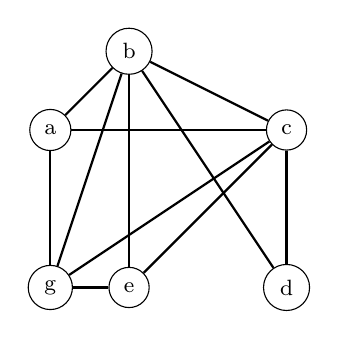
\begin{tikzpicture}
      \begin{scope}[every node/.style={draw=black,circle}]
        \node (a) at ( 0, 1) {\footnotesize e};
        \node (b) at ( 0, 4) {\footnotesize b};
        \node (c) at ( 2, 1) {\footnotesize d};
        \node (d) at ( 2, 3) {\footnotesize c};
        \node (e) at (-1, 1) {\footnotesize g};
        \node (f) at (-1, 3) {\footnotesize a};
      \end{scope}
      \begin{scope}[every edge/.style={draw=black,thick}]
        \path (a) edge (b);
        \path (a) edge (d);
        \path (a) edge (e);
        \path (b) edge (c);
        \path (b) edge (d);
        \path (b) edge (e);
        \path (b) edge (f);
        \path (c) edge (d);
        \path (d) edge (e);           
        \path (d) edge (f);
        \path (e) edge (f);
      \end{scope}
    \end{tikzpicture}
  \end{center}
  \begin{center}
    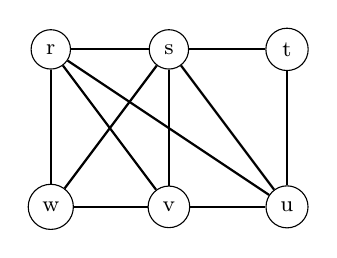
\begin{tikzpicture}
      \begin{scope}[every node/.style={draw=black,circle}]
        \node (a) at (0  ,0) {\footnotesize w};
        \node (b) at (0  ,2) {\footnotesize r};
        \node (c) at (1.5,0) {\footnotesize v};
        \node (d) at (1.5,2) {\footnotesize s};
        \node (e) at (3  ,0) {\footnotesize u};
        \node (f) at (3  ,2) {\footnotesize t};
      \end{scope}
      \begin{scope}[every edge/.style={draw=black,thick}]
        \path (a) edge (b);
        \path (a) edge (c);
        \path (c) edge (e);
        \path (a) edge (d);
        \path (b) edge (c);
        \path (b) edge (d);
        \path (b) edge (e);
        \path (b) edge (d);
        \path (d) edge (f);
        \path (c) edge (d);
        \path (d) edge (e);	            
        \path (e) edge (f);
      \end{scope}
    \end{tikzpicture}
  \end{center}
    
  \section*{No of maps}
    \(f(a) \rightarrow 6\) choices; \(f(b) \rightarrow 5\) choices; \(f(c) \rightarrow 4\) choices; etc.
    So, \(n!\) maps between the vertex sets of two graphs with \(n\) vertices.
  
  \section*{Some invariants}
    \begin{itemize}
      \item Degrees.
      \item Paths.
      \item Connection.
    \end{itemize}

  \section*{Adjacency matrix}
    Fix a listing of \(V\).
    \([a_{ij}]\) where \(a_{ij}\) is 1 if \(\{v_i,v_j\} \in E \) else 0.
  
  \section*{Example}
  \[
    \begin{bmatrix}
      0 & 1 & 1 & 0 & 0 & 1 \\
      1 & 0 & 1 & 1 & 1 & 1 \\
      1 & 1 & 0 & 1 & 1 & 1 \\
      0 & 1 & 1 & 0 & 0 & 0 \\
      0 & 1 & 1 & 0 & 0 & 1 \\
      1 & 1 & 1 & 0 & 1 & 0 
    \end{bmatrix}
    \qquad
    \begin{bmatrix}
      0 & 1 & 0 & 1 & 1 & 1 \\
      1 & 0 & 1 & 1 & 1 & 1 \\
      0 & 1 & 0 & 1 & 0 & 0 \\
      1 & 1 & 1 & 0 & 1 & 0 \\
      1 & 1 & 0 & 1 & 0 & 1 \\
      1 & 1 & 0 & 0 & 1 & 0 \\
    \end{bmatrix}
  \]
  \section*{Encoding}

  %\bibliography{bibliography}
\end{document}